\documentclass[12pt, letterpaper]{article}
\usepackage{graphicx} % Required for inserting images
\usepackage{hyperref}
\usepackage{listings}
\usepackage{amssymb}
\usepackage{amsmath}
\usepackage[english]{babel}
\usepackage{amsfonts}
\usepackage{nicefrac, xfrac}
\usepackage[utf8]{inputenc}
\usepackage{mathtools}
\newcommand{\acc}{\\\hphantom{}\\}
\usepackage[dvipsnames]{xcolor}
\usepackage[titles]{tocloft} % Optional: Better control of the table of contents

\definecolor{light-gray}{gray}{0.95}
\newcommand{\code}[1]{\colorbox{light-gray}{\texttt{#1}}}
\newcommand{\codee}[1]{\colorbox{white}{\texttt{#1}}}
\usepackage[paper=a4paper,left=20mm,right=20mm,bottom=25mm,top=25mm]{geometry}
\renewcommand{\labelenumii}{\arabic{enumi}.\arabic{enumii}}
\renewcommand{\labelenumiii}{\arabic{enumi}.\arabic{enumii}.\arabic{enumiii}}
\renewcommand{\labelenumiv}{\arabic{enumi}.\arabic{enumii}.\arabic{enumiii}.\arabic{enumiv}}
\newcommand{\id}{{\hphantom{ident}}}
\newcommand{\vincolo}[1]{\colorbox{Orange}{$[$\text{#1}$]$}}
\title{\textbf{Progetto}}

\date{}

\begin{document}

\maketitle

\tableofcontents 
\newpage
\section{Requisiti}
\begin{verbatim}
  


\end{verbatim}
\newpage\section{UML}
\begin{center}
    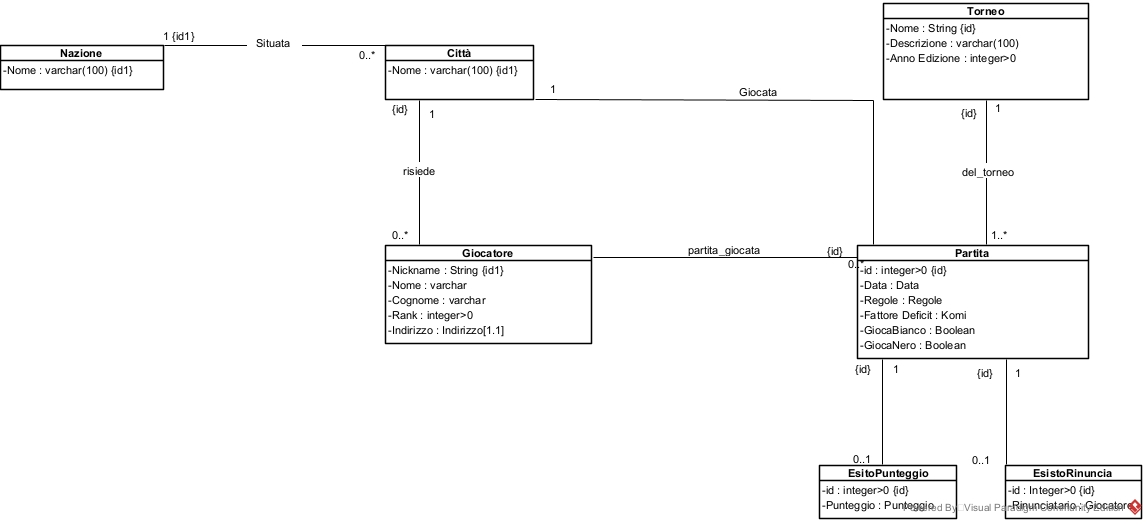
\includegraphics[width=1\textwidth ]{Images/UML.jpg}
\end{center} 
\newpage
\section{Tipi di Dato}


\section{Vincoli Esterni}

\newpage
\section{Specifica Classi}

\section{Use-Case}
\subsection{Diagramma}
\begin{center}
    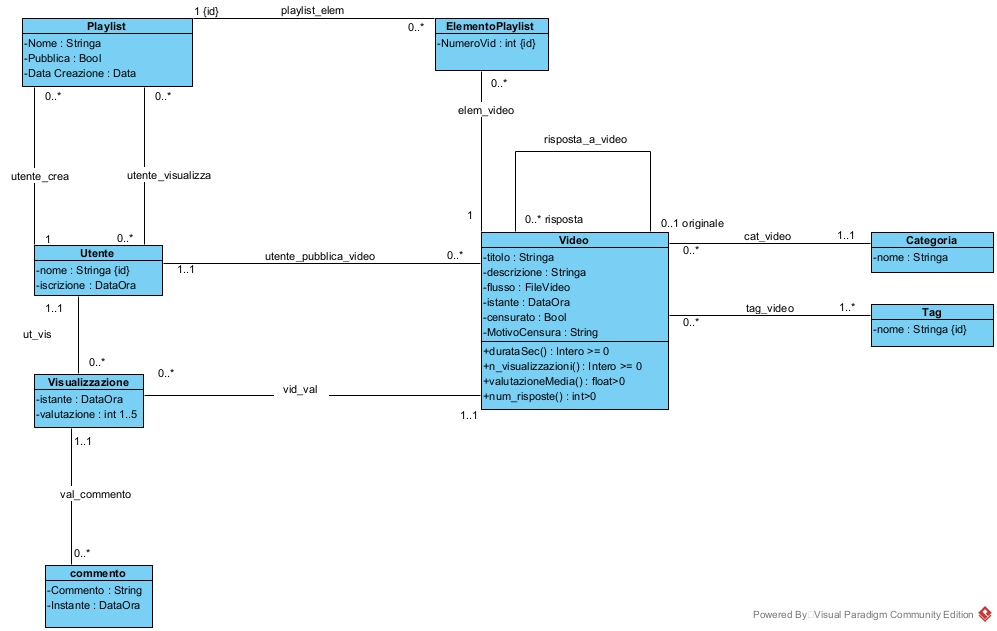
\includegraphics[width=1\textwidth ]{Images/UseCase.jpg}
\end{center} 
\newpage
\subsection{Specifica Use-Case}

    



\newpage
Arrivati a questo punto la fase di \textbf{Analisi} è \textbf{finita}.
\section{Ristrutturazione}
\subsection{Diagramma UML ristrutturato}
\begin{center}
    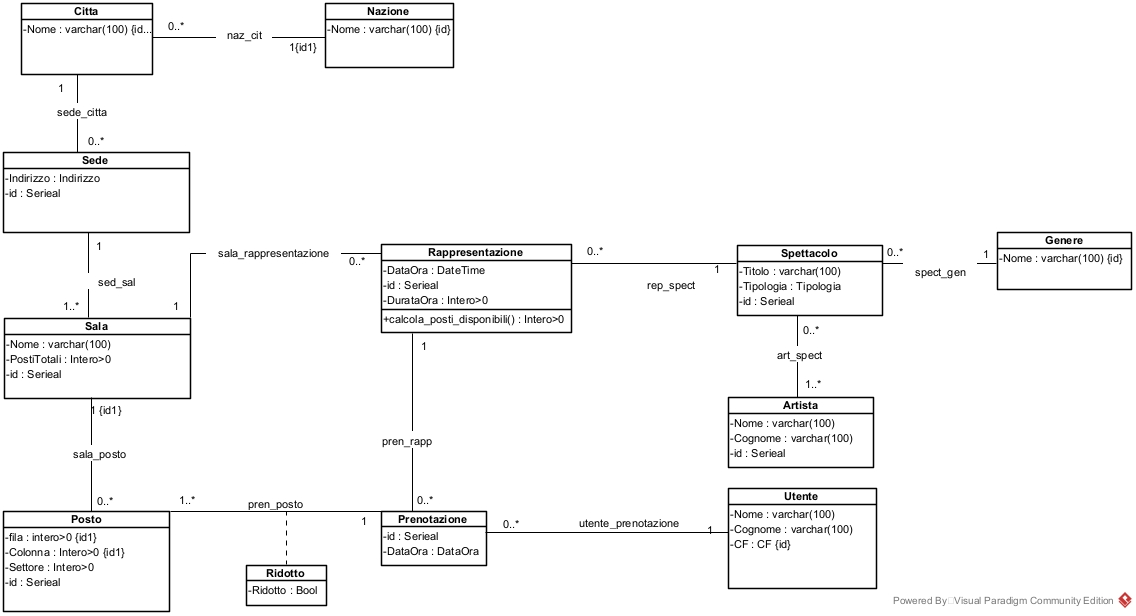
\includegraphics[width=1\textwidth ]{Images/UMLRistrutturato.jpg}
\end{center} 
\newpage
\textbf{Modifiche sulle generalizzazioni effettuate:}\\


\subsection{Tipi e Domini}
\subsubsection{Tipi}

\subsubsection{Domini}

\subsection{Vincoli Esterni}
Non sono stati inseriti nuovi vincoli esterni.
\subsection{Use Case}
Gli use case non violano la nuova ristrutturazione.
\newpage
\subsection{Traduzione diretta del diagramma UML delle classi ristrutturato}
Saranno scritte tutte le tabelle da creare:\\

\newpage \subsection{Trigger}
I vincoli esterni da controllare con i trigger sono:\\

\newpage \subsection{Progettazione Funzionalità}
Le Funzionalità da implementare nella base di dati sono:\\

\end{document}